% Options for packages loaded elsewhere
\PassOptionsToPackage{unicode}{hyperref}
\PassOptionsToPackage{hyphens}{url}
%
\documentclass[
]{book}
\usepackage{lmodern}
\usepackage{amsmath}
\usepackage{ifxetex,ifluatex}
\ifnum 0\ifxetex 1\fi\ifluatex 1\fi=0 % if pdftex
  \usepackage[T1]{fontenc}
  \usepackage[utf8]{inputenc}
  \usepackage{textcomp} % provide euro and other symbols
  \usepackage{amssymb}
\else % if luatex or xetex
  \usepackage{unicode-math}
  \defaultfontfeatures{Scale=MatchLowercase}
  \defaultfontfeatures[\rmfamily]{Ligatures=TeX,Scale=1}
\fi
% Use upquote if available, for straight quotes in verbatim environments
\IfFileExists{upquote.sty}{\usepackage{upquote}}{}
\IfFileExists{microtype.sty}{% use microtype if available
  \usepackage[]{microtype}
  \UseMicrotypeSet[protrusion]{basicmath} % disable protrusion for tt fonts
}{}
\makeatletter
\@ifundefined{KOMAClassName}{% if non-KOMA class
  \IfFileExists{parskip.sty}{%
    \usepackage{parskip}
  }{% else
    \setlength{\parindent}{0pt}
    \setlength{\parskip}{6pt plus 2pt minus 1pt}}
}{% if KOMA class
  \KOMAoptions{parskip=half}}
\makeatother
\usepackage{xcolor}
\IfFileExists{xurl.sty}{\usepackage{xurl}}{} % add URL line breaks if available
\IfFileExists{bookmark.sty}{\usepackage{bookmark}}{\usepackage{hyperref}}
\hypersetup{
  pdftitle={Wood Anatomy of Puerto Rican Trees},
  pdfauthor={Silvia Bibbo, Kasia Ziemińska, Robert Muscarella},
  hidelinks,
  pdfcreator={LaTeX via pandoc}}
\urlstyle{same} % disable monospaced font for URLs
\usepackage{color}
\usepackage{fancyvrb}
\newcommand{\VerbBar}{|}
\newcommand{\VERB}{\Verb[commandchars=\\\{\}]}
\DefineVerbatimEnvironment{Highlighting}{Verbatim}{commandchars=\\\{\}}
% Add ',fontsize=\small' for more characters per line
\usepackage{framed}
\definecolor{shadecolor}{RGB}{248,248,248}
\newenvironment{Shaded}{\begin{snugshade}}{\end{snugshade}}
\newcommand{\AlertTok}[1]{\textcolor[rgb]{0.94,0.16,0.16}{#1}}
\newcommand{\AnnotationTok}[1]{\textcolor[rgb]{0.56,0.35,0.01}{\textbf{\textit{#1}}}}
\newcommand{\AttributeTok}[1]{\textcolor[rgb]{0.77,0.63,0.00}{#1}}
\newcommand{\BaseNTok}[1]{\textcolor[rgb]{0.00,0.00,0.81}{#1}}
\newcommand{\BuiltInTok}[1]{#1}
\newcommand{\CharTok}[1]{\textcolor[rgb]{0.31,0.60,0.02}{#1}}
\newcommand{\CommentTok}[1]{\textcolor[rgb]{0.56,0.35,0.01}{\textit{#1}}}
\newcommand{\CommentVarTok}[1]{\textcolor[rgb]{0.56,0.35,0.01}{\textbf{\textit{#1}}}}
\newcommand{\ConstantTok}[1]{\textcolor[rgb]{0.00,0.00,0.00}{#1}}
\newcommand{\ControlFlowTok}[1]{\textcolor[rgb]{0.13,0.29,0.53}{\textbf{#1}}}
\newcommand{\DataTypeTok}[1]{\textcolor[rgb]{0.13,0.29,0.53}{#1}}
\newcommand{\DecValTok}[1]{\textcolor[rgb]{0.00,0.00,0.81}{#1}}
\newcommand{\DocumentationTok}[1]{\textcolor[rgb]{0.56,0.35,0.01}{\textbf{\textit{#1}}}}
\newcommand{\ErrorTok}[1]{\textcolor[rgb]{0.64,0.00,0.00}{\textbf{#1}}}
\newcommand{\ExtensionTok}[1]{#1}
\newcommand{\FloatTok}[1]{\textcolor[rgb]{0.00,0.00,0.81}{#1}}
\newcommand{\FunctionTok}[1]{\textcolor[rgb]{0.00,0.00,0.00}{#1}}
\newcommand{\ImportTok}[1]{#1}
\newcommand{\InformationTok}[1]{\textcolor[rgb]{0.56,0.35,0.01}{\textbf{\textit{#1}}}}
\newcommand{\KeywordTok}[1]{\textcolor[rgb]{0.13,0.29,0.53}{\textbf{#1}}}
\newcommand{\NormalTok}[1]{#1}
\newcommand{\OperatorTok}[1]{\textcolor[rgb]{0.81,0.36,0.00}{\textbf{#1}}}
\newcommand{\OtherTok}[1]{\textcolor[rgb]{0.56,0.35,0.01}{#1}}
\newcommand{\PreprocessorTok}[1]{\textcolor[rgb]{0.56,0.35,0.01}{\textit{#1}}}
\newcommand{\RegionMarkerTok}[1]{#1}
\newcommand{\SpecialCharTok}[1]{\textcolor[rgb]{0.00,0.00,0.00}{#1}}
\newcommand{\SpecialStringTok}[1]{\textcolor[rgb]{0.31,0.60,0.02}{#1}}
\newcommand{\StringTok}[1]{\textcolor[rgb]{0.31,0.60,0.02}{#1}}
\newcommand{\VariableTok}[1]{\textcolor[rgb]{0.00,0.00,0.00}{#1}}
\newcommand{\VerbatimStringTok}[1]{\textcolor[rgb]{0.31,0.60,0.02}{#1}}
\newcommand{\WarningTok}[1]{\textcolor[rgb]{0.56,0.35,0.01}{\textbf{\textit{#1}}}}
\usepackage{longtable,booktabs}
\usepackage{calc} % for calculating minipage widths
% Correct order of tables after \paragraph or \subparagraph
\usepackage{etoolbox}
\makeatletter
\patchcmd\longtable{\par}{\if@noskipsec\mbox{}\fi\par}{}{}
\makeatother
% Allow footnotes in longtable head/foot
\IfFileExists{footnotehyper.sty}{\usepackage{footnotehyper}}{\usepackage{footnote}}
\makesavenoteenv{longtable}
\usepackage{graphicx}
\makeatletter
\def\maxwidth{\ifdim\Gin@nat@width>\linewidth\linewidth\else\Gin@nat@width\fi}
\def\maxheight{\ifdim\Gin@nat@height>\textheight\textheight\else\Gin@nat@height\fi}
\makeatother
% Scale images if necessary, so that they will not overflow the page
% margins by default, and it is still possible to overwrite the defaults
% using explicit options in \includegraphics[width, height, ...]{}
\setkeys{Gin}{width=\maxwidth,height=\maxheight,keepaspectratio}
% Set default figure placement to htbp
\makeatletter
\def\fps@figure{htbp}
\makeatother
\setlength{\emergencystretch}{3em} % prevent overfull lines
\providecommand{\tightlist}{%
  \setlength{\itemsep}{0pt}\setlength{\parskip}{0pt}}
\setcounter{secnumdepth}{5}
\usepackage{booktabs}
\usepackage{amsthm}
\makeatletter
\def\thm@space@setup{%
  \thm@preskip=8pt plus 2pt minus 4pt
  \thm@postskip=\thm@preskip
}
\makeatother
\ifluatex
  \usepackage{selnolig}  % disable illegal ligatures
\fi
\usepackage[]{natbib}
\bibliographystyle{apalike}

\title{Wood Anatomy of Puerto Rican Trees}
\author{Silvia Bibbo, Kasia Ziemińska, Robert Muscarella}
\date{2021-05-19}

\begin{document}
\maketitle

{
\setcounter{tocdepth}{1}
\tableofcontents
}
\hypertarget{introduction}{%
\chapter*{Introduction}\label{introduction}}
\addcontentsline{toc}{chapter}{Introduction}

\hypertarget{species-list}{%
\chapter*{Species list}\label{species-list}}
\addcontentsline{toc}{chapter}{Species list}

\textbf{\protect\hyperlink{araliaceae}{Araliaceae}}

\begin{itemize}
\tightlist
\item
  \protect\hyperlink{schefflera-morototoni}{\emph{Schefflera morototoni}}
\end{itemize}

\textbf{\protect\hyperlink{bursuraceae}{Bursuraceae}}

\begin{itemize}
\tightlist
\item
  \protect\hyperlink{dacryodes-excelsa}{\emph{Dacryodes excelsa}}
\item
  \protect\hyperlink{tetragastris-balsamifera}{\emph{Tetragastris balsamifera}}
\end{itemize}

\textbf{\protect\hyperlink{elaeocarpaceae}{Elaeocarpaceae}}

\begin{itemize}
\tightlist
\item
  \protect\hyperlink{sloanea-berteroana}{\emph{Sloanea berteroana}}
\end{itemize}

\textbf{\protect\hyperlink{fabaceae}{Fabaceae}}

\begin{itemize}
\tightlist
\item
  \protect\hyperlink{inga-laurina}{\emph{Inga laurina}}
\end{itemize}

\textbf{\protect\hyperlink{salicaceae}{Salicaceae}}

\begin{itemize}
\tightlist
\item
  \protect\hyperlink{casearia-arborea}{\emph{Casearia arborea}}
\end{itemize}

\textbf{\protect\hyperlink{sapindaceae}{Sapindaceae}}

\begin{itemize}
\tightlist
\item
  \protect\hyperlink{matayba-domingensis}{\emph{Matayba domingensis}}
\end{itemize}

\textbf{\protect\hyperlink{sapotaceae}{Sapotaceae}}

\begin{itemize}
\tightlist
\item
  \protect\hyperlink{manilkara-bidentata}{\emph{Manilkara bidentata}}
\end{itemize}

\textbf{\protect\hyperlink{urticaceae}{Urticaceae}}

\begin{itemize}
\tightlist
\item
  \protect\hyperlink{cecropia-schreberiana}{\emph{Cecropia schreberiana}}
\end{itemize}

\hypertarget{methods}{%
\chapter*{Methods}\label{methods}}
\addcontentsline{toc}{chapter}{Methods}

Here we describe the methods, from field to data.

\hypertarget{sample-collection}{%
\section*{Sample collection}\label{sample-collection}}
\addcontentsline{toc}{section}{Sample collection}

Collecting samples for wood anatomical analysis requires careful consideration of the research questions or objectives.

\begin{itemize}
\tightlist
\item
  Sample size
\item
  Position of sample
\item
  Other data to record
\end{itemize}

\textbf{Additional Resources}

\begin{itemize}
\tightlist
\item
  reference 1
\item
  reference 2
\item
  \ldots{}
\end{itemize}

\hypertarget{sectioning-and-slide-preparation}{%
\section*{Sectioning and slide preparation}\label{sectioning-and-slide-preparation}}
\addcontentsline{toc}{section}{Sectioning and slide preparation}

\begin{figure}

{\centering 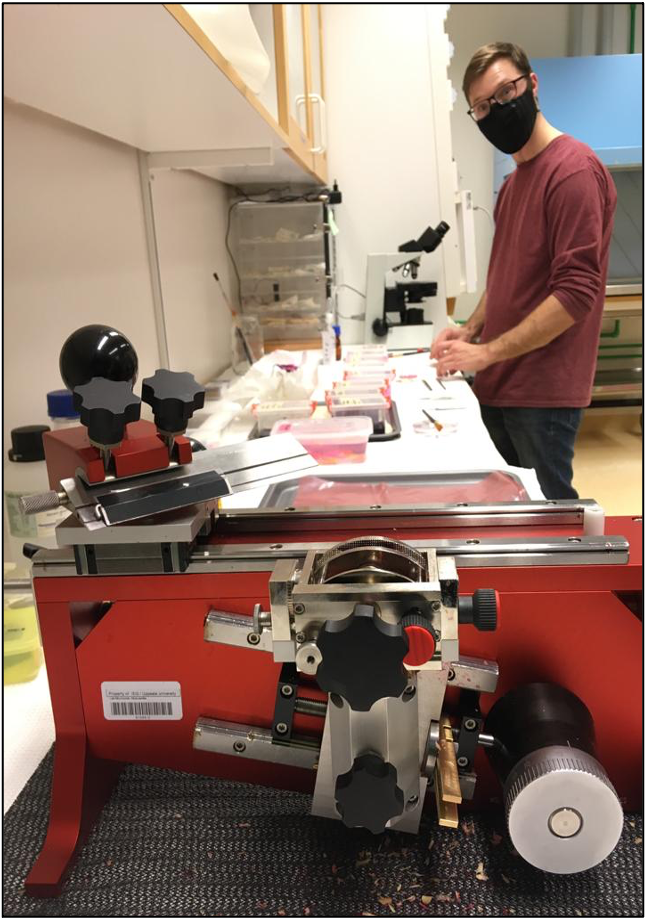
\includegraphics[width=8.96in,height=0.4\textheight]{images/Methods/sectioning/sam} 

}

\caption{Sectioning samples with the WSL lab microtome.}\label{fig:unnamed-chunk-3}
\end{figure}

\hypertarget{image-capture}{%
\section*{Image capture}\label{image-capture}}
\addcontentsline{toc}{section}{Image capture}

\begin{figure}

{\centering 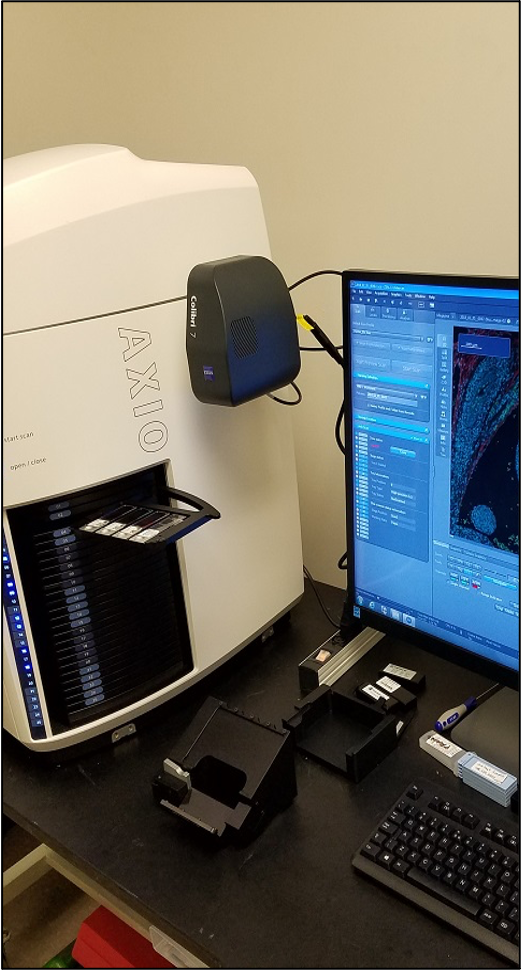
\includegraphics[width=7.25in,height=0.4\textheight]{images/Methods/imaging/scan} 

}

\caption{Scanning slides with the Zeiss slide scanner.}\label{fig:unnamed-chunk-4}
\end{figure}

\hypertarget{image-analysis}{%
\section*{Image analysis}\label{image-analysis}}
\addcontentsline{toc}{section}{Image analysis}

Details on the protocol\ldots{}

\begin{itemize}
\tightlist
\item
  \href{https://qupath.github.io/}{\texttt{QuPath}}
\end{itemize}

\hypertarget{processing-of-annotated-images-in-r}{%
\section*{Processing of annotated images in R}\label{processing-of-annotated-images-in-r}}
\addcontentsline{toc}{section}{Processing of annotated images in R}

We have developed the \texttt{qwar} R package to process the annotated images (as .svg files). You can see the \href{https://github.com/bobmuscarella/qwar}{source code on Github} and install the package like this:

\begin{Shaded}
\begin{Highlighting}[]
\FunctionTok{library}\NormalTok{(devtools)}
\NormalTok{devtools}\SpecialCharTok{::}\FunctionTok{install\_github}\NormalTok{(}\StringTok{"bobmuscarella/qwar"}\NormalTok{)}
\end{Highlighting}
\end{Shaded}

Some examples of possible outputs from the \texttt{qwar} R package are shown below.

\begin{figure}

{\centering 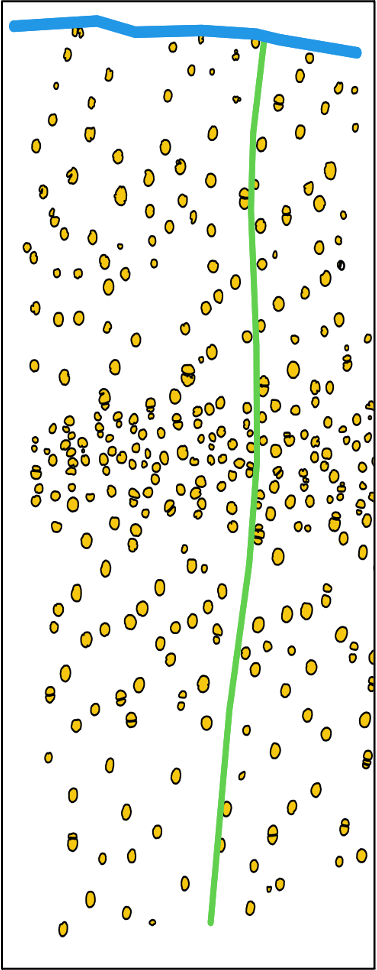
\includegraphics[width=5.24in,height=0.2\textheight]{images/Methods/r/vessels} 

}

\caption{An example of output from the `qwar` R package.}\label{fig:unnamed-chunk-6}
\end{figure}

\begin{figure}

{\centering 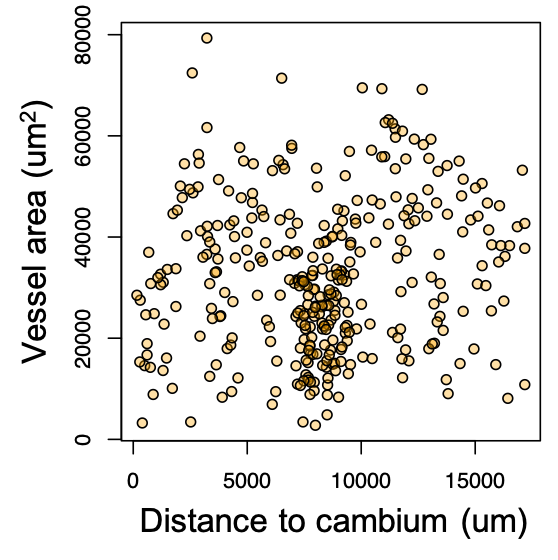
\includegraphics[width=7.75in,height=0.4\textheight]{images/Methods/r/graph} 

}

\caption{Quantifying vessel area as a function of distance to cambiumusing the `qwar` R package.}\label{fig:unnamed-chunk-7}
\end{figure}

\hypertarget{araliaceae}{%
\chapter{Araliaceae}\label{araliaceae}}

Species in Araliaceae

\hypertarget{schefflera-morototoni}{%
\section*{\texorpdfstring{\emph{Schefflera morototoni}}{Schefflera morototoni}}\label{schefflera-morototoni}}
\addcontentsline{toc}{section}{\emph{Schefflera morototoni}}

\hypertarget{bignoniaceae}{%
\chapter{Bignoniaceae}\label{bignoniaceae}}

Species in Bignoniaceae

\hypertarget{tabebuia-heterophylla}{%
\section*{\texorpdfstring{\emph{Tabebuia heterophylla}}{Tabebuia heterophylla}}\label{tabebuia-heterophylla}}
\addcontentsline{toc}{section}{\emph{Tabebuia heterophylla}}

\hypertarget{bursuraceae}{%
\chapter{Bursuraceae}\label{bursuraceae}}

Species in Bursuraceae

\hypertarget{dacryodes-excelsa}{%
\section*{\texorpdfstring{\emph{Dacryodes excelsa}}{Dacryodes excelsa}}\label{dacryodes-excelsa}}
\addcontentsline{toc}{section}{\emph{Dacryodes excelsa}}

\emph{Longitudinal sections}

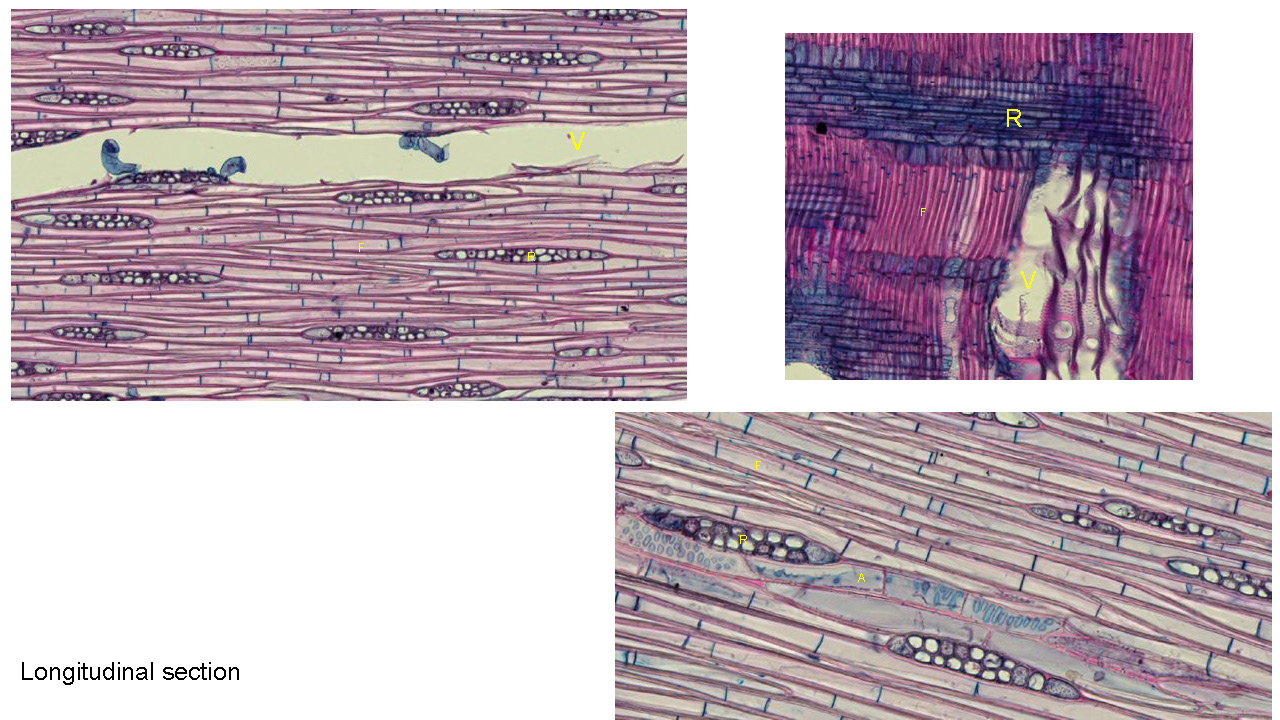
\includegraphics{images/DACEXC/2021-03-10_Image_reference_library.pptx_Page_20.jpg}
\emph{Cross sections}

\begin{figure}
\centering
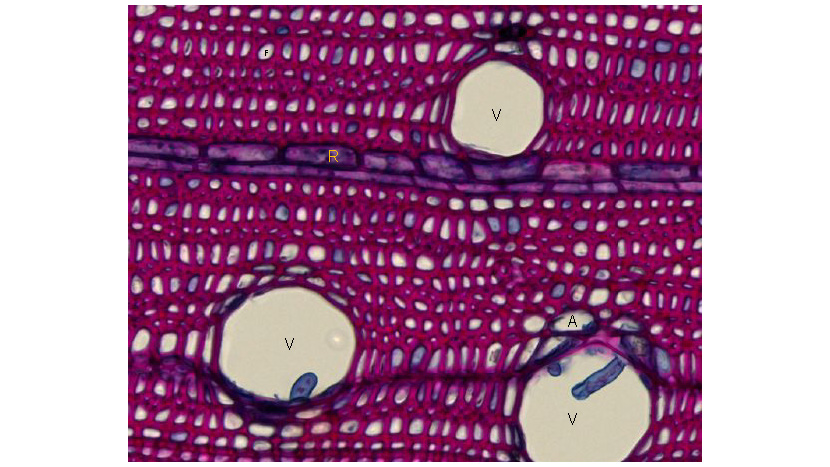
\includegraphics{2021-03-10_Image_reference_library.pptx_Page_21.jpg}
\caption{Dacryodes excelsa cross 1}
\end{figure}

\hypertarget{tetragastris-balsamifera}{%
\section*{\texorpdfstring{\emph{Tetragastris balsamifera}}{Tetragastris balsamifera}}\label{tetragastris-balsamifera}}
\addcontentsline{toc}{section}{\emph{Tetragastris balsamifera}}

\hypertarget{elaeocarpaceae}{%
\chapter{Elaeocarpaceae}\label{elaeocarpaceae}}

Species in Elaeocarpaceae

\hypertarget{sloanea-berteroana}{%
\section*{\texorpdfstring{\emph{Sloanea berteroana}}{Sloanea berteroana}}\label{sloanea-berteroana}}
\addcontentsline{toc}{section}{\emph{Sloanea berteroana}}

\hypertarget{fabaceae}{%
\chapter{Fabaceae}\label{fabaceae}}

Species in Fabaceae

\hypertarget{inga-laurina}{%
\section*{\texorpdfstring{\emph{Inga laurina}}{Inga laurina}}\label{inga-laurina}}
\addcontentsline{toc}{section}{\emph{Inga laurina}}

\hypertarget{salicaceae}{%
\chapter{Salicaceae}\label{salicaceae}}

Species in Salicaceae

\hypertarget{casearia-arborea}{%
\section*{\texorpdfstring{\emph{Casearia arborea}}{Casearia arborea}}\label{casearia-arborea}}
\addcontentsline{toc}{section}{\emph{Casearia arborea}}

\begin{figure}

{\centering 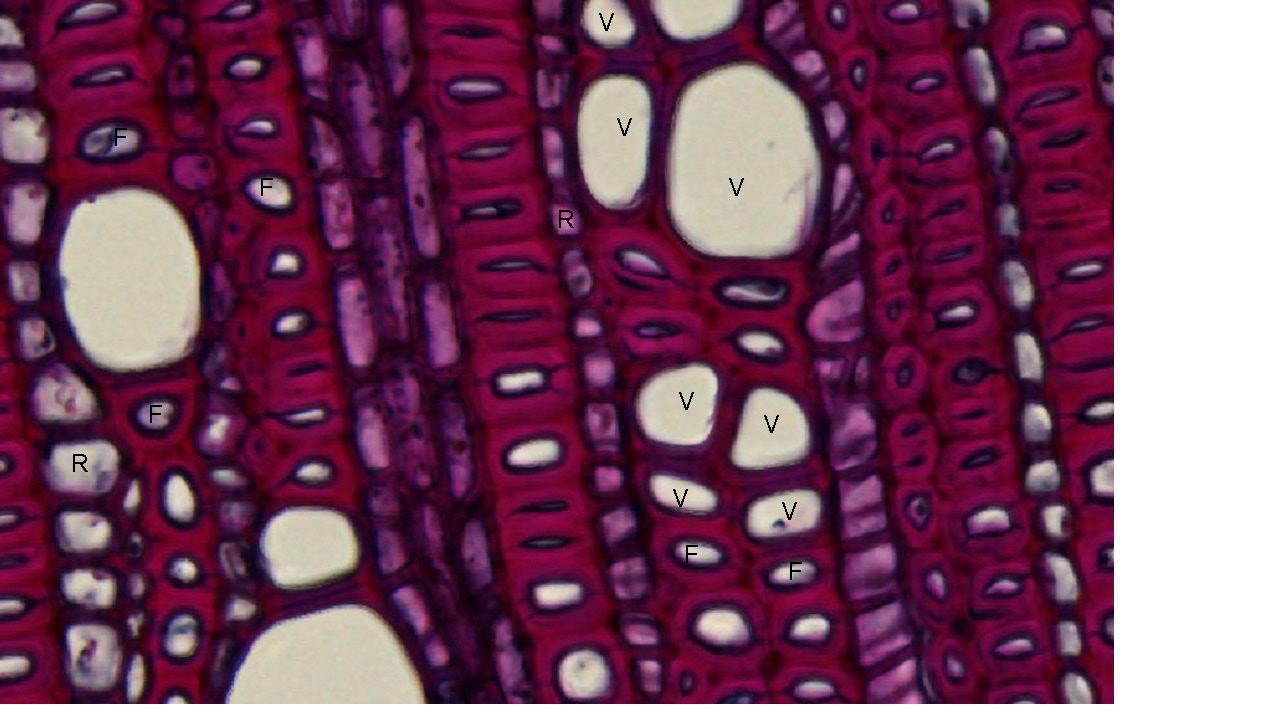
\includegraphics[width=17.78in,height=0.4\textheight]{images/CASARB/2021-03-10_Image_reference_library.pptx_Page_04} 

}

\caption{Figure caption}\label{fig:unnamed-chunk-11}
\end{figure}

\hypertarget{sapindaceae}{%
\chapter{Sapindaceae}\label{sapindaceae}}

Species in Sapindaceae

\hypertarget{matayba-domingensis}{%
\section*{\texorpdfstring{\emph{Matayba domingensis}}{Matayba domingensis}}\label{matayba-domingensis}}
\addcontentsline{toc}{section}{\emph{Matayba domingensis}}

\hypertarget{sapotaceae}{%
\chapter{Sapotaceae}\label{sapotaceae}}

Species in Sapotaceae

\hypertarget{manilkara-bidentata}{%
\section*{\texorpdfstring{\emph{Manilkara bidentata}}{Manilkara bidentata}}\label{manilkara-bidentata}}
\addcontentsline{toc}{section}{\emph{Manilkara bidentata}}

\hypertarget{urticaceae}{%
\chapter{Urticaceae}\label{urticaceae}}

Species in Urticaceae

\hypertarget{cecropia-schreberiana}{%
\section*{\texorpdfstring{\emph{Cecropia schreberiana}}{Cecropia schreberiana}}\label{cecropia-schreberiana}}
\addcontentsline{toc}{section}{\emph{Cecropia schreberiana}}

  \bibliography{packages.bib}

\end{document}
